% 56 x 36 inch C2C poster summarizing completed work only.
% Compile from docs/posters with:
%   pdflatex -interaction=nonstopmode jma_c2c_poster.tex
\documentclass[final]{beamer}
\usepackage[orientation=landscape,size=custom,width=142.24,height=91.44,scale=1.18]{beamerposter}
\usepackage[T1]{fontenc}
\usepackage{helvet}
\renewcommand{\familydefault}{\sfdefault}
\usepackage{booktabs}
\usepackage{array}
\usepackage{graphicx}
\usepackage{ragged2e}
\usepackage{tikz}
\usetikzlibrary{arrows.meta,positioning,shapes.geometric}

\definecolor{HopkinsBlue}{HTML}{002D72}
\definecolor{HopkinsNavy}{HTML}{17375E}
\definecolor{LightBlue}{HTML}{E8F0F8}
\definecolor{EAOrange}{HTML}{E67E22}
\definecolor{BarcodeRed}{HTML}{BE3737}
\definecolor{NormalGreen}{HTML}{37824B}
\definecolor{BodyGray}{HTML}{333333}

\setbeamercolor{background canvas}{bg=white}
\setbeamercolor{normal text}{fg=BodyGray,bg=white}
\setbeamercolor{block title}{fg=white,bg=HopkinsBlue}
\setbeamercolor{block body}{fg=BodyGray,bg=white}
\setbeamertemplate{navigation symbols}{}
\setbeamertemplate{blocks}[rounded][shadow=false]
\setbeamertemplate{itemize item}{\color{HopkinsBlue}$\blacktriangleright$}
\setbeamertemplate{itemize subitem}{\color{HopkinsBlue}$\bullet$}
\setlength{\columnsep}{1.3cm}
\setlength{\columnseprule}{0pt}
\setbeamerfont{block title}{series=\bfseries,size=\Large}
\setbeamerfont{block body}{size=\large}

\graphicspath{{assets/}{../../results/manual_ground_truth/}{../../results/automatic_detector/}}
\newcommand{\EA}{\textcolor{EAOrange}{\textbf{EA}}}
\newcommand{\Barcode}{\textcolor{BarcodeRed}{\textbf{barcoding}}}
\newcommand{\Normal}{\textcolor{NormalGreen}{\textbf{normal}}}

\begin{document}
\begin{frame}[t]

% Fixed-coordinate header reproduces the supplied Hopkins poster template.
\makebox[\linewidth][c]{%
\begin{tikzpicture}[x=1cm,y=1cm]
  \path[use as bounding box] (0,0) rectangle (142.24,13.5);
  \fill[HopkinsBlue] (0,0) rectangle (142.24,13.5);
  \node[inner sep=0pt] at (8.5,7.4)
    {
\includegraphics[width=12.0cm]{jhu_whiting_white.png}};
  \node[inner sep=0pt] at (133.74,7.4)
    {
\includegraphics[width=12.0cm]{jhu_whiting_white.png}};
  \node[text=white,text width=108cm,align=center] at (71.12,10.1)
    {{\fontsize{52}{58}\selectfont\bfseries
      Quantifying the ``Barcoding'' Artifact in OCT for EA Progression Risk}};
  \node[text=white,text width=112cm,align=center] at (71.12,7.4)
    {{\fontsize{20}{24}\selectfont\bfseries
      Jonathan Ma, Yingjia Wei\textsuperscript{*,1,2},
      Hussein Morobeid, MD\textsuperscript{*,3,4}, Karen Daynes\textsuperscript{3},
      Steffen Schmitz-Valckenberg, MD\textsuperscript{3,4},
      Monika Fleckenstein, MD\textsuperscript{3}}};
  \node[text=white,text width=112cm,align=center] at (71.12,5.25)
    {{\fontsize{13}{16}\selectfont
      \textsuperscript{1}Johns Hopkins University-Whiting School of Engineering, Baltimore, MD, USA $\mid$
      \textsuperscript{2}Department of Population Health Science, School of
      Medicine, University of Utah, Salt Lake City, UT, USA}};
  \node[text=white,text width=112cm,align=center] at (71.12,3.45)
    {{\fontsize{13}{16}\selectfont
      \textsuperscript{3}John A. Moran Eye Center, University of Utah,
      Salt Lake City, UT, USA $\mid$
      \textsuperscript{4}Department of Ophthalmology, University of Bonn,
      Bonn, Germany}};
  \node[text=white,align=center] at (71.12,1.75)
    {{\fontsize{13}{16}\selectfont
      \href{mailto:jonathanma217@outlook.com}{jonathanma217@outlook.com}
      $\mid$ \href{https://jonathanma03.github.io}{jonathanma03.github.io}}};
\end{tikzpicture}}

\vspace{1.0cm}
\begin{columns}[t,totalwidth=\dimexpr\paperwidth-4cm\relax]

% LEFT COLUMN ---------------------------------------------------------------
\begin{column}{0.285\textwidth}
  \begin{block}{Clinical Motivation}
    Early atrophy (EA) is an important precursor to advanced atrophic change
    in age-related macular degeneration (AMD). Clinicians have also observed a
    vertical hypertransmission pattern in baseline OCT, informally called
    \Barcode, which is believed to mark regions at greater risk of subsequent
    progression.

    \vspace{0.4cm}
    Barcoding has no standardized quantitative definition. Visual assessment
    is difficult to reproduce at scale, motivating an interpretable method to
    localize and measure both barcoding and EA at baseline.
  \end{block}

  \begin{block}{Completed Preprocessing}
    \begin{enumerate}
      \item Load a selected B-scan and scanner-provided segmentation metadata from a HEYEX E2E volume.
      \item Flatten the scan to BM and retain 150 pixels below it.
      \item Standardize the retained region within each scan using a z-score.
      \item Apply mild Gaussian denoising $(1.0,0.5)$ while preserving vertical patterns.
    \end{enumerate}
    These operations place scans into a comparable anatomical coordinate
    system while retaining the sub-BM signal used by the detector.
  \end{block}

  \begin{block}{Features and Interpretation}
    % \small
    Features are robustly standardized relative to the same scan:
    \[
      z_F(x)=\frac{F(x)-\operatorname{median}(F)}
      {\operatorname{IQR}(F)+\epsilon}.
    \]
    \textbf{Intensity.} Column median $M(x)$ represents typical
    hypertransmission, while the 90th percentile $Q(x)$ captures the brightest
    relevant pixels.

    \textbf{Depth continuity.} Horizontal patterns in a local window are
    correlated between rows separated by the selected lag $d=4$:
    \[
      C(x)=\frac{1}{D-d}\sum_{y=1}^{D-d}
      \operatorname{corr}(\mathbf I_{y,x},\mathbf I_{y+d,x}).
    \]
    High continuity means that bright and dark locations stay aligned deeper
    into the scan.

    \textbf{Verticality.} Smoothed gradients form a structure tensor
    $\mathbf J$. Its eigenvalues and dominant orientation produce
    \[
      V(x)=\frac{\lambda_1-\lambda_2}
      {\lambda_1+\lambda_2+\epsilon}\cos^2\theta.
    \]
    The first term measures directional organization; $\cos^2\theta$ asks
    whether that direction agrees with a vertical line. Larger $V$ therefore
    indicates a stronger vertical structure.

    \textbf{Gabor texture.} Quadrature filters measure repeating vertical
    bright--dark patterns at wavelengths $\lambda=4,8,16$ pixels:
    \[
      G_\lambda(x)=\operatorname{mean}_y
      \sqrt{(I*g_\lambda^c)^2+(I*g_\lambda^s)^2}.
    \]

    The calibrated models use $[M,Q,C,V]$ plus 
    interactions after LRT. Positive interaction evidence means two visible properties
    jointly support a phenotype more strongly than either property alone.
  \end{block}
\end{column}

% CENTER COLUMN -------------------------------------------------------------
\begin{column}{0.39\textwidth}
  \begin{block}{Model Framework}
    \vspace{1.0cm}
    \centering
    \begin{tikzpicture}[
      every node/.style={font=\normalsize,align=center},
      stage/.style={draw=HopkinsBlue,very thick,rounded corners=5pt,
        fill=LightBlue,minimum height=2.4cm,text width=5.8cm},
      ea/.style={stage,draw=EAOrange,fill=EAOrange!10},
      barcode/.style={stage,draw=BarcodeRed,fill=BarcodeRed!10},
      reject/.style={stage,draw=gray!75,fill=gray!10},
      final/.style={stage,draw=NormalGreen,fill=NormalGreen!10},
      arrow/.style={-{Latex[length=5mm]},very thick,draw=HopkinsNavy}]
      \node[stage] (scan) at (0,0) {Processed \\B-scan};
      \node[stage] (features) at (7.5,0) {M, Q, C, V,\\MQ, CV, QC, QV};
      \node[ea] (eascore) at (15.0,3.0) {EA \\model};
      \node[barcode] (bcscore) at (15.0,-3.0) {Barcoding \\model};
      \node[reject] (veto) at (23.0,0) {Local context +\\structural veto};
      \node[barcode] (confirm) at (31.0,0) {Texture +\\near-depth confirmation};
      \node[final] (output) at (39.0,0) {Final intervals\\\Normal{} / \EA{} / \Barcode};
      \draw[arrow] (scan)--(features);
      \draw[arrow] (features)--(eascore);
      \draw[arrow] (features)--(bcscore);
      \draw[arrow] (eascore)--(veto);
      \draw[arrow] (bcscore)--(veto);
      \draw[arrow] (veto)--(confirm);
      \draw[arrow] (confirm)--(output);
    \end{tikzpicture}

    \vspace{0.35cm}
    \justifying
    Separate calibrated logistic models score EA and barcoding. Local support,
    interval probability, feature votes, minimum width, and gap filling remove
    isolated responses. A structural model and dark-shadow rule reject likely
    vessels or anatomy. Gabor and near-depth gates provide additional
    confirmation only for barcoding.

    \vspace{0.35cm}
    \textbf{Current Calibrated Specification.}
    {%\small
    \begin{columns}[t,totalwidth=\linewidth]
      \begin{column}{0.49\linewidth}
        \textcolor{BarcodeRed}{\textbf{Barcoding}}
        \begin{itemize}
          \item At least 55\% local support within $\pm5$ columns
          \item Interval mean/peak probability $\geq0.52/0.68$
          \item At least two feature votes
          \item Minimum width 8; maximum bridged gap 4
          \item Gabor texture and near-depth confirmation
        \end{itemize}
      \end{column}
      \begin{column}{0.49\linewidth}
        \textcolor{EAOrange}{\textbf{Early Atrophy (EA)}}
        \begin{itemize}
          \item At least 60\% local support within $\pm7$ columns
          \item Interval mean/peak probability $\geq0.48/0.62$
          \item At least three feature votes
          \item Minimum width 12; maximum bridged gap 5
          \item No Gabor-texture or depth-band gate
        \end{itemize}
      \end{column}
    \end{columns}
    }
    \vspace{1.0cm}
    \justifying
    A candidate is retained when it demonstrates sufficiently strong
    vertical-pattern energy together with increased brightness near Bruch's
    membrane. Hypertransmission is evaluated across near (0--20\%), middle
    (20--50\%), and deep (50--100\%) sub-BM regions to characterize how the
    signal persists with depth. 
  \end{block}

  \begin{block}{Segmentation Results}
    \vspace{0.3cm}
    \textbf{Strongest Barcoding Case (Fast)}
    \begin{columns}[t,totalwidth=\linewidth]
      \begin{column}{0.49\linewidth}
        \centering
        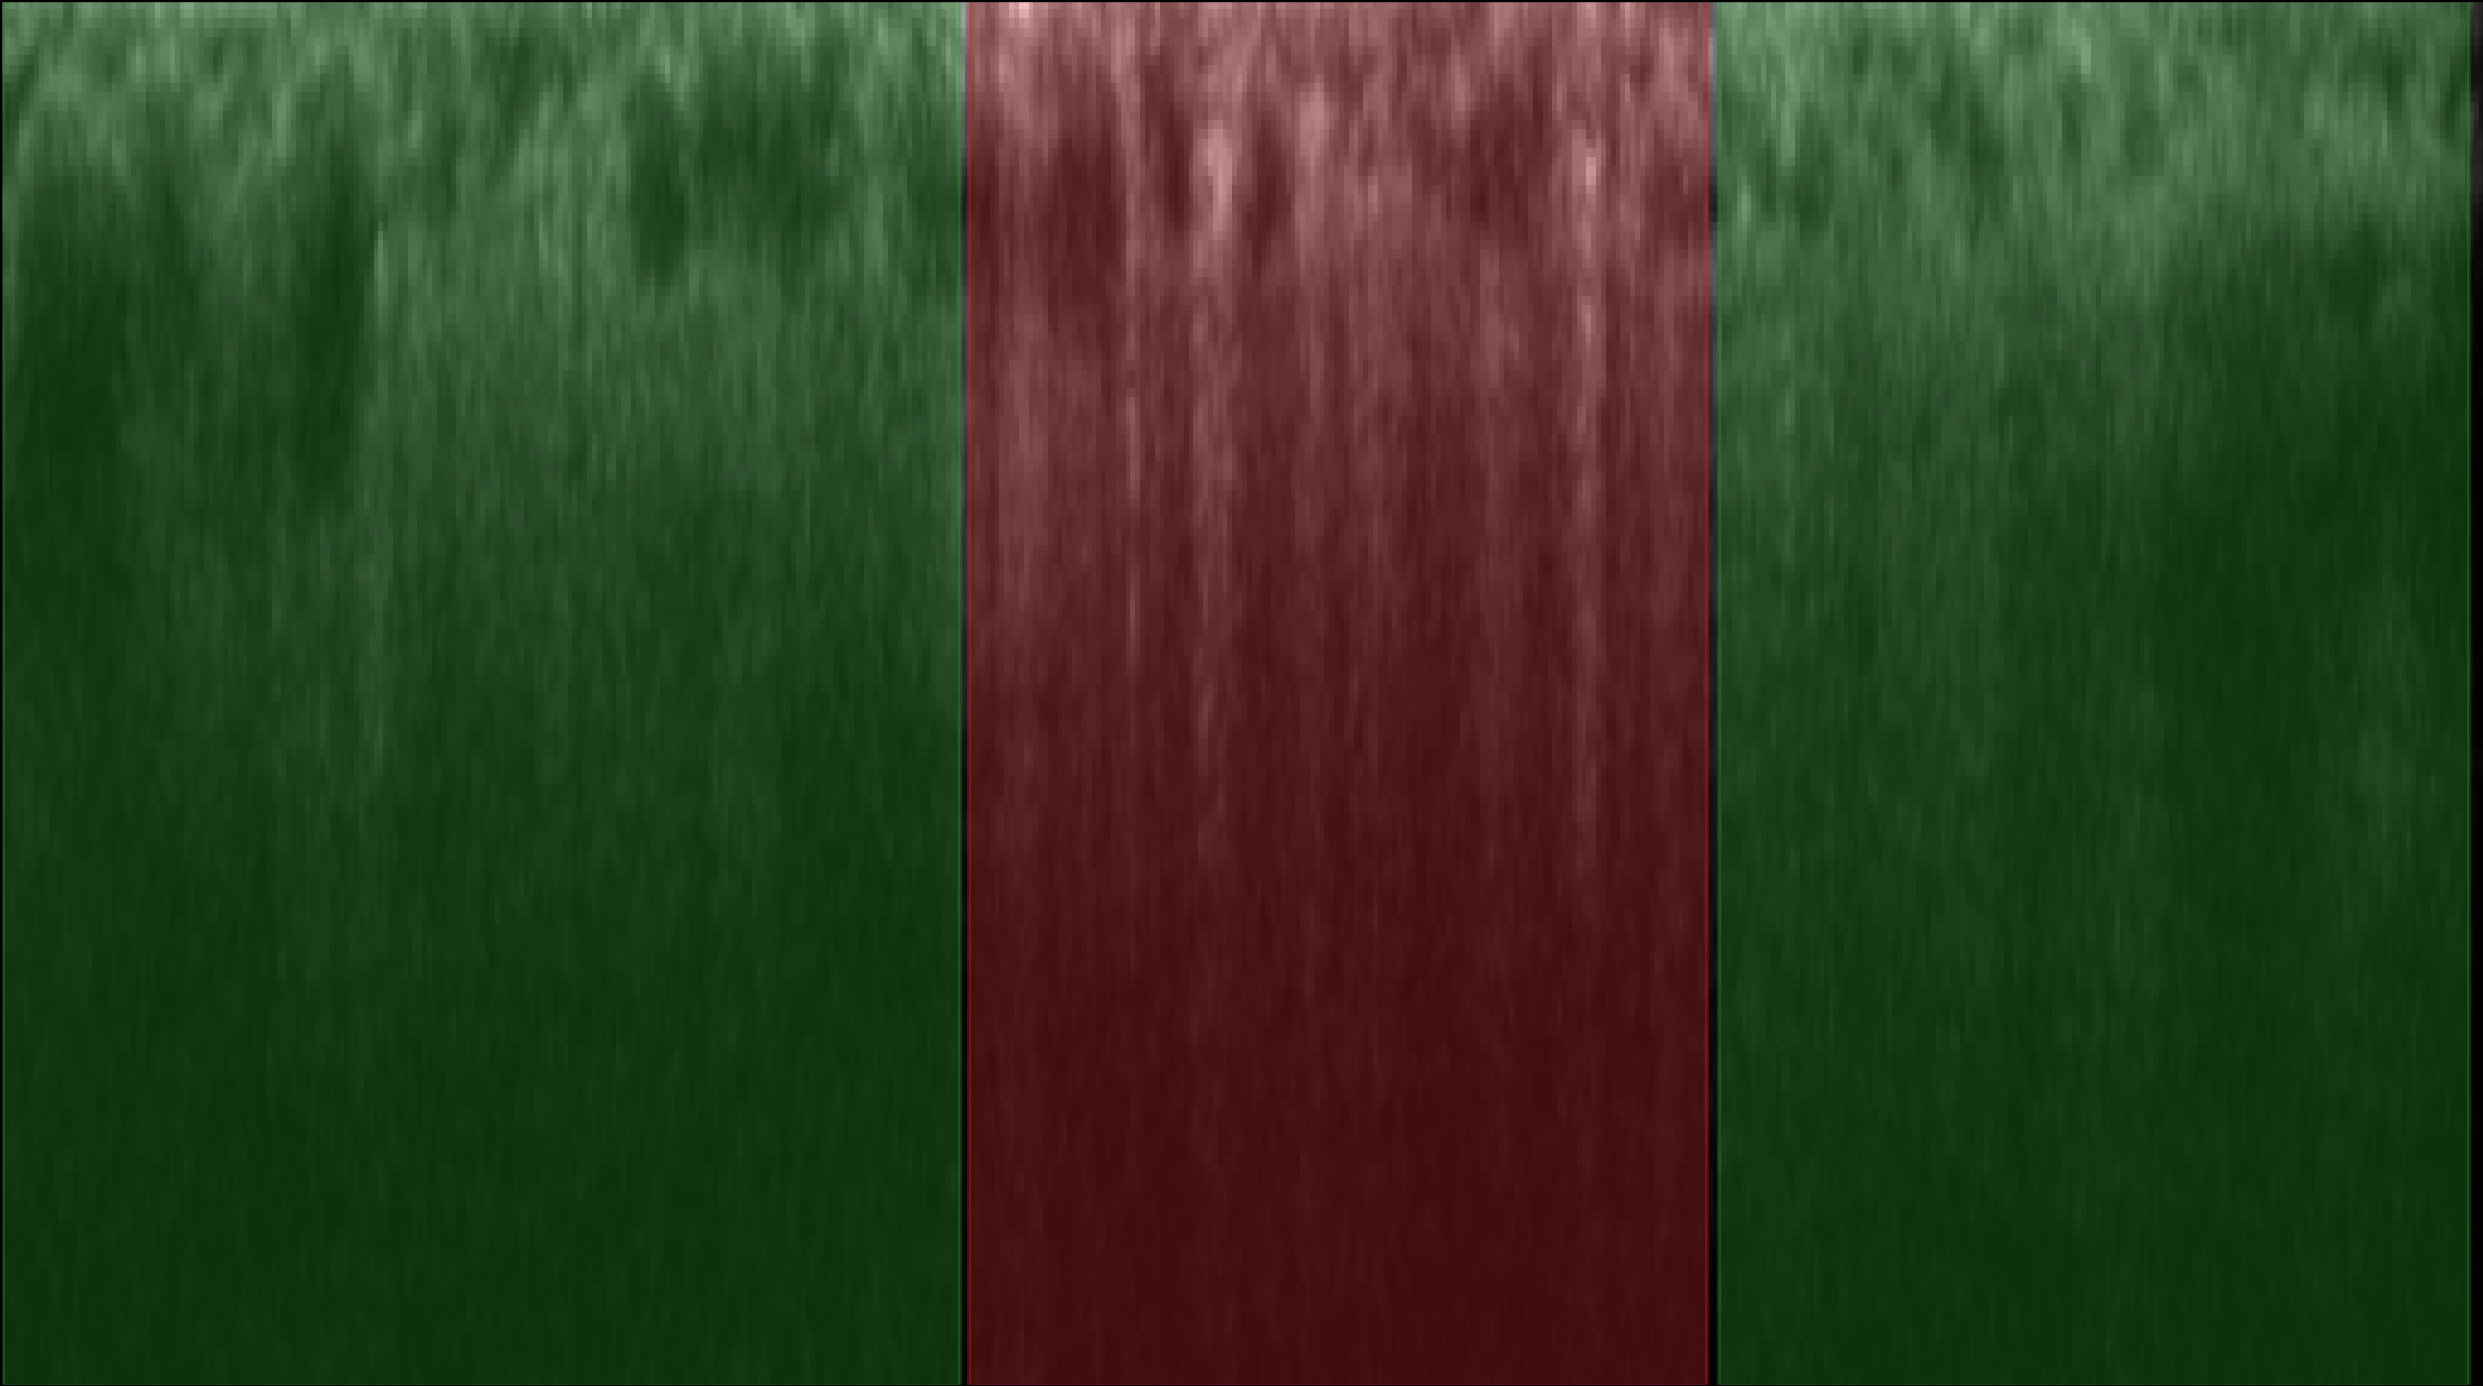
\includegraphics[width=\linewidth,height=7.2cm]{fast_49_bscan_033_ground_truth.png}

        \textbf{Ground Truth}
      \end{column}
      \begin{column}{0.49\linewidth}
        \centering
        
\includegraphics[width=\linewidth,height=7.2cm]{fast_49_bscan_033_automatic.png}

        \textbf{Detector Output}
      \end{column}
    \end{columns}

    \centering
    \vspace{0.3cm}
    Barcoding precision 0.92, recall 0.71, Dice 0.81.

    \vspace{0.35cm}
    \justifying
    \textbf{Strongest EA Case (Slow)}
    \begin{columns}[t,totalwidth=\linewidth]
      \begin{column}{0.49\linewidth}
        \centering
        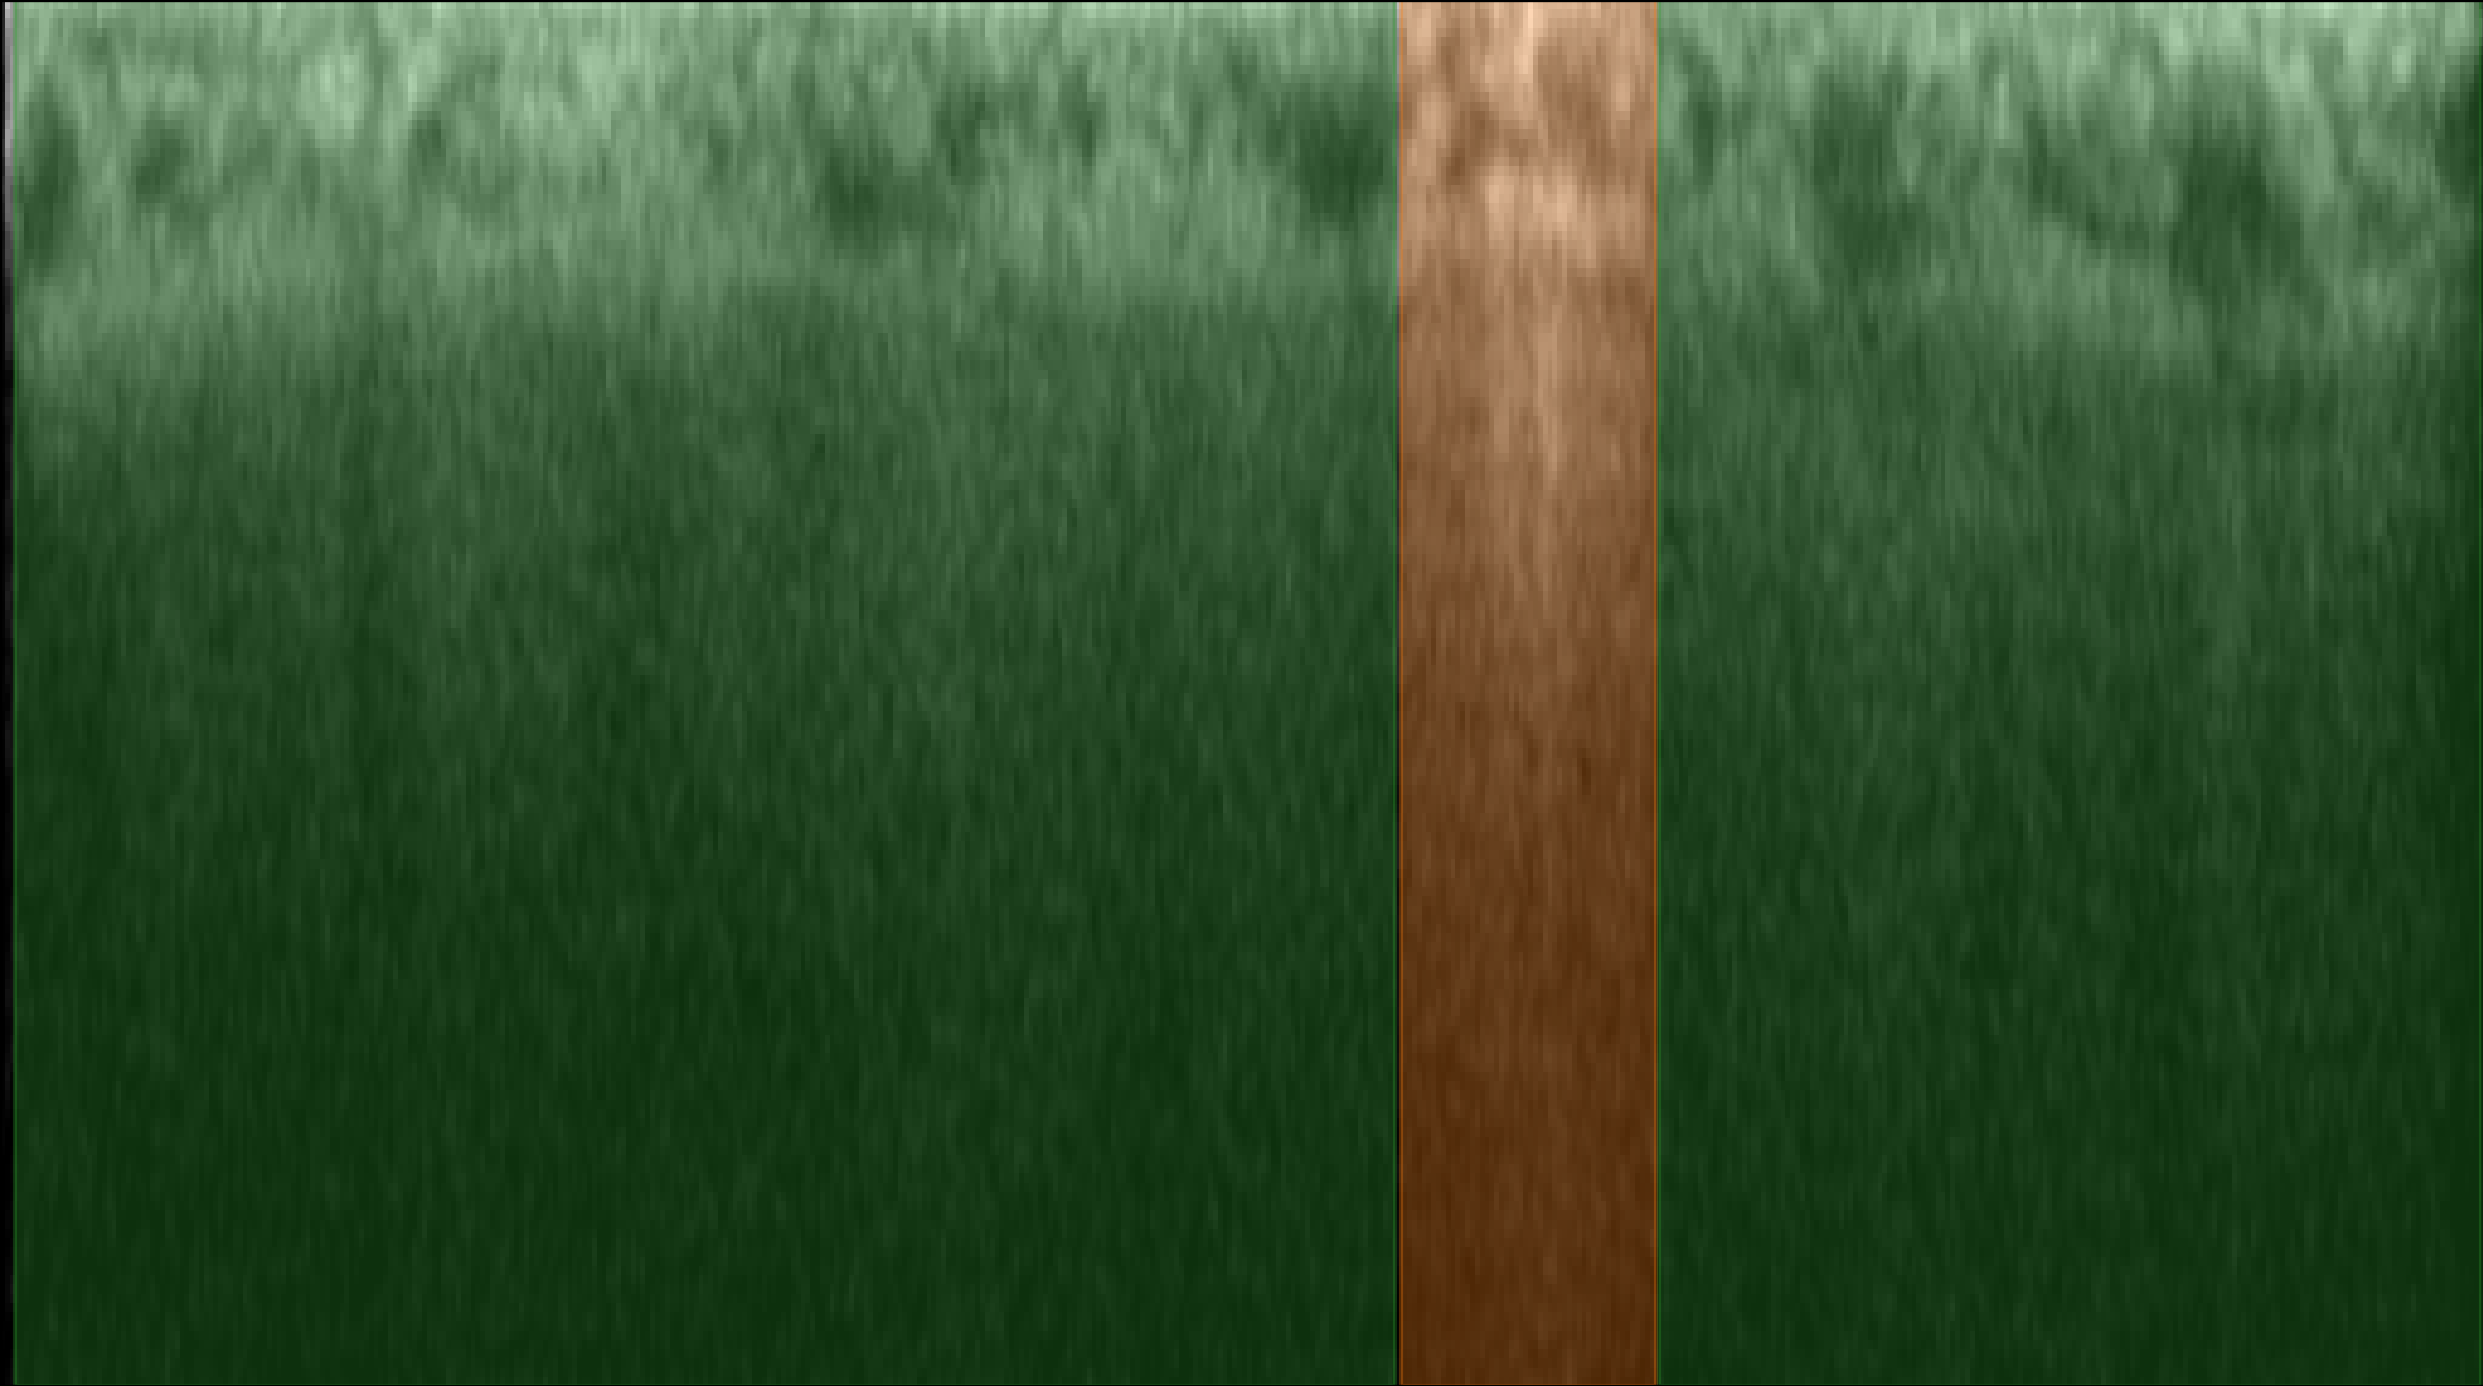
\includegraphics[width=\linewidth,height=7.2cm]{slow_47_bscan_031_ground_truth.png}

        \textbf{Ground Truth}
      \end{column}
      \begin{column}{0.49\linewidth}
        \centering
        
\includegraphics[width=\linewidth,height=7.2cm]{slow_47_bscan_031_automatic.png}

        \textbf{Detector Output}
      \end{column}
    \end{columns}

    \centering
    \vspace{0.3cm}
    EA precision 1.00, recall 0.91, Dice 0.95.

    \justifying
    These cases show the best saved agreement for each phenotype. The fast case closely captured the major barcoding regions; the slow closely reproduced
    the single manual EA interval. Small additional phenotype responses remain visible in both automatic outputs, due to small training size.
  \end{block}

\end{column}

% RIGHT COLUMN --------------------------------------------------------------
\begin{column}{0.295\textwidth}
  \begin{block}{Ten-Scan Validation and Group Agreement}
    \vspace{0.3cm}
    Five manually selected fast-progressor and slow-progressor
    B-scans were loaded from the pipeline and
    compared with manual annotations. Uncertain and vessel/structural columns
    were excluded from scoring.

    \vspace{0.25cm}
    \centering
    \renewcommand{\arraystretch}{1.2}
    \begin{tabular}{lccc}
      \toprule
      \textbf{Detector Output} & \textbf{Precision} & \textbf{Recall} & \textbf{Dice}\\
      \midrule
      Current model: barcoding & 0.817 & 0.520 & 0.636\\
      Current model: EA & 0.462 & 0.699 & 0.557\\
      \bottomrule
    \end{tabular}

    \vspace{0.25cm}
    \justifying
    The two rows are outputs from the same pipeline. Precision measures
    resistance to false alarms, recall measures recovery of manually marked
    tissue, and Dice summarizes overlap.

    \vspace{0.3cm}
    \textbf{Agreement within each five-scan progression group:}
    \vspace{0.3cm}
    \centering
    \renewcommand{\arraystretch}{1.15}
    \begin{tabular}{llccc}
      \toprule
      \textbf{Group} & \textbf{Finding} & \textbf{Prec.} & \textbf{Recall} & \textbf{Dice}\\
      \midrule
      Fast & Barcoding & 0.775 & 0.545 & 0.640\\
      Slow & Barcoding & 0.303 & 0.370 & 0.333\\
      Fast & EA & 0.259 & 0.549 & 0.352\\
      Slow & EA & 0.629 & 0.760 & 0.688\\
      \bottomrule
    \end{tabular}

    \vspace{0.3cm}
    \justifying
    Barcoding agreement was stronger in the selected fast scans, whereas EA
    agreement was stronger in the slow scans. Because these ten selected scans
    informed detector tuning, all values are development results rather than
    independent clinical-validation estimates and cannot establish a biological
    fast-versus-slow difference.
  \end{block}
  \vspace{1.0cm}
  \begin{block}{Results and Future Work}
    \vspace{0.3cm}
    \textbf{Could barcoding be a useful biomarker?} In this ten-scan
    development set, both progression groups had the same number of
    automatically detected barcoding intervals (18 each), but the fast group
    had greater total detected barcoding width (451 versus 321 image columns;
    40.5\% greater mean width per scan). This preliminary pattern suggests that
    \emph{barcoding extent}, rather than interval count alone, may be worth
    testing as a progression biomarker. It is not yet evidence of a clinical
    association because the sample is small, and more scans are being uploaded for the subjects, but confirms the that barcoding is an interesting phenomenon to investigate
  \end{block}
  \vspace{1.0cm}
  \begin{block}{Funding Support}
    {% \small
    NIH Grant \textbf{1R01EY034965-01}; \textbf{UM1TR004409} (Pilot Projects
    and Services/Resources, Utah Clinical and Translational Science Institute);
    \textbf{EY014800} (National Institutes of Health Core Grant, Department of
    Ophthalmology \& Visual Sciences, University of Utah); John A. Moran Award
    to MF and SS-V (Research Salary Support from John A. Moran Eye Center,
    University of Utah); and an Unrestricted Grant from Research to Prevent
    Blindness, New York, NY, to the Department of Ophthalmology \& Visual
    Sciences, University of Utah.
    }
  \end{block}

\end{column}

\end{columns}

\vfill
% Reserved for funding acknowledgments, NIH award number, and required logos.
\makebox[\linewidth][c]{%
\begin{beamercolorbox}[wd=\paperwidth,ht=2.2cm,dp=0.6cm,leftskip=2cm,rightskip=2cm]{block title}
  \strut
\end{beamercolorbox}}

\end{frame}
\end{document}
